% !Mode:: "TeX:UTF-8"
% !TEX program  = xelatex

%\documentclass{cumcmthesis}
\documentclass[withoutpreface,bwprint]{cumcmthesis} %去掉封面与编号页,电子版提交的时候使用。
\usepackage {tikz}
\usetikzlibrary{patterns}
\usepackage{pgfplots}
\pgfplotsset{compat=1.16}
\usepackage{xcolor}
\usepackage{filecontents}
\usepackage{amsmath}
\usetikzlibrary{snakes}
\usepgfplotslibrary{groupplots}
\definecolor{Gray}{RGB}{213,213,213}

\usepackage[framemethod=TikZ]{mdframed}
\usepackage{url}   % 网页链接
\usepackage{subcaption} % 子标题
\title{周期性节律现象建模与实例分析}
\tihao{A}
\baominghao{4321}
\schoolname{华中师范大学}
\membera{姓\quad 名~1}
\memberb{姓\quad 名~2}
\memberc{姓\quad 名~3}
\supervisor{姓\quad 名~1}
\yearinput{2021}
\monthinput{08}
\dayinput{22}

\usepackage{hyperref}
\hypersetup{colorlinks,
          linkcolor = blue,	
          anchorcolor = blue,
          urlcolor = blue,
       citecolor = red,
          }

\begin{document}

 \maketitle

 \begin{abstract}
针对自然界中普遍存在的周期性或近似周期性现象进行了研究。从弹簧振子
模型中抽象出了一个能解释该类现象的常微分方程模型(基本模型),并进行了
详细研究。

首先,对于不考虑阻尼、外界激励的一些简单情况,我们直接给出了模型的
解析解。对于复杂的情况,我们从模型的频域出发,给出了系统的频率响应特性。
从频域的角度,给出了如何利用该模型来阐释产生这些周期性现象的机制,得到
了令人满意的结果。

然后,我们将模型推广到非线性系统的混沌响应中,得到了一个推广模型,
利用它来解释实际系统中产生的一类貌似随机的拟周期现象。在小信号意义下,
该推广模型和基本模型是一致的,这样就实现了基本模型和推广模型之间的完美
统一。

最后,我们以当前正在广泛研究的智能电网技术为契机,结合其中的一个研
究分支—可再生能源发电技术,给出如何将我们的模型用来描述分布式可再生
能源并网技术中的接口——微电网。以该实际系统为背景,我们进行了详细的讨
论,利用所提模型分析了该系统中各种形式的周期性和拟周期性现象的产生机
理。验证了我们模型的有效性和正确性。特别地,还讨论了系统在某些特定条件
下所呈现的混沌现象。同时,我们还给出了模型结果的实际物理意义。
此外,还给出了模型的客观评价和进一步工作的展望。

\keywords{周期性和拟周期性现象;反馈机制和激励机制;常微分方程模型;分岔;
混沌;微电网}

%%%%%%%%%%%%%%%%%%%%%%%%%%%%%%%%%%%%%%%%%%%%%%%%
%% 运用时这部分删除
%% =============================================
\vfill

%\hfill
%\begin{minipage}{0.3\linewidth}
%  \centering{\includegraphics[width=\linewidth]{gongzhonghao}}\\[-5pt]
%  \href{http://www.latexstudio.net}{更多\LaTeX{} 模板资源下载}
%\end{minipage}
%% =============================================

\end{abstract}

%目录  2019 明确不要目录,我觉得这个规定太好了
%\tableofcontents

%\newpage

\section{问题重述}
\label{sec1}

周期性或近似周期性(拟周期性)现象是一类普遍存在的现象,在自然界的
生命体或者人工智能系统中,可以发现有许多的此类现象存在。这些周期节律的
现象会根据自身内部的反馈机制以及外界的刺激或者外界输入的变化而变化:(A)
或者节律变快了,但是振幅变化不太大;(B)或者振幅变化很大,但是节律相对
稳定;(C)亦或者两者都会有较大的变化。以下我们分别称这三种现象为:A 类、
B 类和 C 类现象,例如,正常人的心跳节律在有无外界刺激时就会有 A 类现象
的出现;正常人和病人的体温昼夜变化又会有 B 类现象的出现。问:

%\begin{enumerate}
  %\item
 (1) 请设计若干数学模型,以便能够充分反映上述描述的这些节律现象,并解
释模型产生这些现象的机制。

  %\item
 (2) 考虑将设计的模型具体运用于某一个具有实际背景的系统中,并评价模型
的优点和缺点。
%\end{enumerate}

\section{问题分析}
\label{sec2}

在这里,我们给出实际系统中周期性和拟周期性现象的定义。随后,将混沌
现象看作是拟周期性现象的极端,简单介绍了混沌现象的工程背景。然后,以线
性反馈和共振现象为例,分析了反馈机制和外界激励是如何影响系统行为演化的。

\subsection{周期性和拟周期性}
\label{sec2-1}

所谓的周期性是指:存在一个时间 $T$, 使得  $\boldsymbol{x}(t)=\boldsymbol{x}(t+T) $, 其中,  $\boldsymbol{x} \in \boldsymbol{R}^{n} $ 是
动力系统 $ \dot{x}=f(x, t) $ 的轨线。当 $ f $ 显含时间 $ t$  时,动力系统称为非自治系统, 否 则称为自治系统。当然, 这里的周期性也包括多周期的情况, 即 $ T \in \boldsymbol{U} \subset \boldsymbol{R}^{+}, \boldsymbol{U} $
即为所有可能在周期的集合。然而,并不是所有的系统都会呈现严格的周期性, 大量的实际系统所表现出来的只是近似的周期现象,更确切地说是一种“拟周期 性”。这种貌似周期性的现象,在很长的一段时期内困扰着工程技术人员。首先, 很难获取精确的解析解; 齐次,从数值上难于解释其机理,尤其是当系统的反圆 机制进一步增强或外界激励达到一定阀值时, 这种拟周期行为甚至会演化为一种 貌似随机的现象一混屯。 1963 年, Lorenz发现了对流现象中的周期流会朝着不规则沛流演化的规律~\upcite{1} 从此, 确定性系统中的混屯现象开始被人们接受。在该理论中, 如果将周期 解或平衡点视作系统的一个稳态解的话, 那么所谓的近似周期解有可能是通向混 屯的一个中介而已。其后,Rossler在Lorenz系统的基础上构造了一个更加简单的 混屯系统模型~\upcite{2}。 1983 年, Leon O. Chua发现了Chua电路~\upcite{3},这是一个真正便于 物理实现的混屯系统,并有严格的数学证明,数值仿真和实验模拟都得到了相同 的结论。该电路的提出具有重要的工程意义,因为它提醒我们工程实践中一些以 前认为是噪声造成的现象或所谓的近似周期现象, 可能是由于确定系统中的混屯 产生的。

\subsection{是什么在影响系统行为的演化?}
\label{sec2-2}

考虑微分动力系统
\begin{align}
\label{eq1}
\begin{cases}
\dot{\bm x}=f({\bm x}, t)+{\bm u} \\
y=h({\bm x})
\end{cases}
\end{align}
其中, $ \boldsymbol{x} \in \boldsymbol{R}^{n} $ 为状态变量; 向量函数 $ \boldsymbol{f}$: $\boldsymbol{R}^{n} \rightarrow \boldsymbol{R}^{n}$, $h$: $\boldsymbol{R}^{n} \rightarrow \boldsymbol{R} $; $y$  为输出变量;
 $\boldsymbol{u} \in \boldsymbol{R}^{n}$  为控制量。

 1、反债:反圆在自动控制系统中得到了广泛的应用,从瓦特在蒸汽机上实 现了闭环反圆控制之后, 各种反圆控制策略成为实现动力系统朝着人们预期目标 演化的一个最重要措施之一~\upcite{4}
 对于式所示的系统, 若 $ \boldsymbol{u}=\boldsymbol{u}(\boldsymbol{x})=-\boldsymbol{K} \boldsymbol{x} $ 就构成了最简单的反圆比例反圆控制
 律。其他,诸如非线性控制、滑模控制、鲁棒控制等,无非是控制向量的函数变 得更加复杂一些罢了, 但是它们应用的基本思想都是一样的,那就是利用系统状 态变量的信息来调节系统的演化方向, 使其朝着人们预期的方向发展。

 2、激励:反圆是一种改变系统行为最普遍的方法, 但是我们不应该忘记激 励的作用。其中,共振是最典型的例子,通过改变外界输入量,当其与系统的固 有模态相匹配的时候可能达到令人意想不到的效果。在工程实际中, 人们利用了 共振的这一原理, 设计了滤波器。人们甚至, 发现了电力系统中的强迫振荡现象, 当负荷扰动满足一定频率时,系统的功率会出现强迫振荡现象,严重时可能导致 系统的解列而带来大停电事故,这是令人毛骨柬然的~\upcite{5}。

\section{符号说明}
\label{sec3}

$x$:  系统的状态变量, $ x_{*}$  为其平衡点,  $x_{0} $ 为其初始值;

$u$:  系统的输入控制量;

$f$:  系统的阻尼, 单位: $ \mathrm{N} $;

$F_{s}$:  弹簧振子的回复力, 单位: $ \mathrm{N} $;

$m$:  弹簧振子中滑块的质量, 单位: $ \mathrm{kg} $;

$k$:  弹簧振子中弹簧的劲度系数,单位:$  \mathrm{N} / \mathrm{m} $;

$\omega_{0}$  : 系统的无阻尼共振角频率, 单位: $ \mathrm{rad} / \mathrm{s} $;

$\omega_{d}$:  系统的有阻尼共振角频率, 单位: $ \mathrm{rad} / \mathrm{s} $;

$D$:  系统的阻尼系数;

$\xi$:系统响应的阻尼比;

$Q$:  品质因素; 注:还有其他一些局部变量,在使用时再加以说明。

\section{模型的建立与求解}
\label{sec4}

对于周期性现象,最好的解释是振动理论。一个最简单的且具有明确物理背
景的现象是弹簧振子问题。对于光滑水平面上一受弹簧约束的滑块,质量为 $m$,
系统的物理模型如图~\ref{fig1} 所示,其动力学方程可由牛顿第二定律得到
\begin{align}
\label{eq2}
m \ddot{x}+f+F_{s}=u
\end{align}
其中,  $x $ 为滑块相对于平衡位置的位移; $ F_{s} $ 为弹簧的回复力; $ f $ 为滑块所受到的 粘滞阻力, 一般 $ f=f(x, \dot{x}) $, 这里可以认为是系统状态变量自身的一种反圆机制; $ u  $为外力,这里可以认为是外界的激励机制。我们知道当位移 $ x$  较小时,可以认 为弹簧的回复力与位移 $ x $ 之间满足线性关系 $ F_{s}=k x$, $k $ 为弹簧的劲度系数。其实, 这里的变量 $ k $, 描述的也是系统自身的一种反圆机制。

%f1
\begin{figure}[h!t]
  \centering
  {
  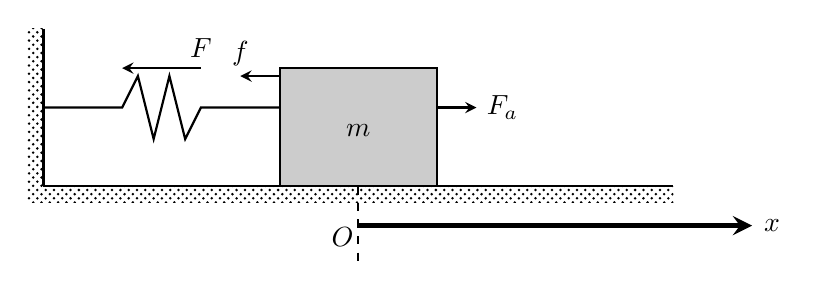
\begin{tikzpicture}[thick]
% ground
\draw [black] (-4,0) -- (4,0);
\fill [pattern = crosshatch dots,
    pattern color = black] (-4,0) rectangle (4,-.2);
\draw [black] (-4,2) -- (-4,0);
\fill [pattern = crosshatch dots,
    pattern color = black] (-4.2,-.2) rectangle (-4,2);
% cart
\begin{scope} [draw = black,
    fill = black!20,
    dot/.style = {black, radius = .025}]
\coordinate [pos = .5] (T) -- (-.09,1.5);
\filldraw (-1,1.5) -- coordinate [pos = .5] (F)
    (-1,0) -- node [above = 0.5cm] {$m$}
    (1,0) -- (1,1.5)
    coordinate (X) -- (.1,1.5)
    arc (0:0:.1) -- (-1.014,1.5);
\end{scope}
    \draw [stealth-] (-3,1.5) --(-2,1.5)node [above] {$F$};
    \draw [-stealth] (-1,1.4) --(-1.5,1.4)node [above] {$f$};
    \draw [-stealth] (1,1) --(1.5,1)node [right] {$F_a$};
     \draw [-stealth,line width=2pt] (0,-0.5) --(5,-0.5)node [right] {${\bm x}$};
    \draw[dashed,thick]  (0,0) --(0,-1)node [left=0.2cm,above=0.1cm] {$O$};
    \draw (-4,1) --(-3,1)--(-2.8,1.4)--(-2.6,0.6)--(-2.4,1.4)--(-2.2,0.6)--(-2,1)--(-1,1);
\end{tikzpicture}
  }
  \caption{弹簧振子的物理模型}\label{fig1}
\end{figure}

对于式~\eqref{eq2} 所示模型,是一个最简单的具有周期解或拟周期解的数学模型~\upcite{6}。
但是,该模型包含了大量的信息,在机械、电力等领域具有广泛的应用~\upcite{7,8,9,10,11}。我
们将在下面的部分做一些详细的分析,讨论系统的参数是如何反映系统的节律现
象的。并利用该模型阐释现实中大量存在的A类、B类和C类周期性或拟周期性现
象的产生机制。

\subsection{无反馈机制和激励机制的情况}
\label{sec4-1}

首先,让我们来考虑一类最简单的情况。这类情况虽然是最简单、最理想的
情况,但是,却有利于我们在~\ref{sec4-2} 中分析系统的反馈机制和激励机制在系统周期
性节律中的作用。在这里所讨论的一类情况中,我们假设系统中不存在粘滞阻力。
同时,我们也不考虑系统的外界激励,此时系统的动力学方程变为
\begin{align}
    \label{eq3}
    m \ddot{x}+kx_{s}=0
    \end{align}
 这是最简单的的弹簧振子的情况。若系统的初始条件为 $ \dot{x}(0)=c_{1}$, $x(0)=c_{2} $, 那么式~\eqref{eq2} 所示方程存在解析解
\begin{align}
\label{eq4}
x(t)=c_{1} \sqrt{m / k} \sin \left(\omega_{0} t\right)+c_{2} \cos \left(\omega_{0} t\right)
\end{align}
其中, $ \omega_{0}=\sqrt{k / m} $ 为系统的无阻尼共振角频率,可由系统的特征方程 $ m \lambda^{2}+k=0 $ 得到, $ \lambda_{1,2}=\pm j \omega_{0}  $。 从式~\eqref{eq4} 可以看出, 当系统存在初始扰动时,由于没有外 加激励和自身的反贵机制,系统将永远不停地做等幅振荡。此外,可以看出系统 的初始速度控制正弦振荡项,而初始位移控制着余弦振荡项。

\subsection{含阻尼和外加激励的情况}
\label{sec4-2}

 现在我们来分析系统的自身反圆和外界激励时如何影响系统的周期性节律
的。首先,我们在方程的基础上考虑系统存在粘滞阻力的作用,且该阻尼正比于 滑块的运动速度, 即 $ f=D \dot{x} $, 同时计及作用在滑块上的外力为周期性激励 $ u=F_{0} \cos (\gamma t) $ 。 那么, 系统的动力学方程变为
\begin{align}
\label{eq5}
m \ddot{x}+D \dot{x}+k x=F_{0} \cos (\gamma t)
\end{align}
其中,  $D $ 为系统的阻尼系数; $ \gamma $ 为外力的周期; $ F_{0} $ 为外力的幅值。通过计算可 以发现,系统仍然存在解析解。一个简单的情况是:不考虑初始速度,只考虑初 始位移, 即初始条件为 $ \dot{x}(0)=0 $ 、  $x(0)=x_{0}  $。 此时。问题的解析解为
\begin{align}
\label{eq6}
x(t)&=\frac{x_{0}\left(4 k m-D \sqrt{D^{2}-4 k m}-D^{2}\right)}{2\left(4 k m-D^{2}\right)}\times\notag\\
&\quad~\bigg({\rm e}^{0.5 t /\left(\left(D-\sqrt{D^{2}-4 k m}\right) m\right)}+{\rm e}^{0.5 t /\left(\left(D+\sqrt{D^{2}-4 k m}\right) m\right)}\bigg)
\end{align}
其中, 值得指出的是:一般地  $D^{2}<4$~km, 故上式是一个复指数方程,其解仍然 是带有振荡的。系统的振荡模态可由其特征方程~\eqref{eq7} 式得到。
\begin{align}
\label{eq7}
m \lambda^{2}+D \lambda+k=0
\end{align}
其解为
\begin{align}
\label{eq8}
\lambda_{1,2}=\frac{-D \pm \sqrt{D^{2}-4 k m}}{2 m}=-\frac{D}{2 m} \pm \sqrt{\left(\frac{D}{2 m}\right)^{2}-\frac{k}{m}}
\end{align}

和~\ref{sec4-1} 中的结果相比,此时的振荡项中带有了阻尼,后面我们将做详细分析。但
是,即使是一个简化的情况(不计外界激励和初始速度),其解的形式都过于复
杂,不便于对问题本质的分析和讨论,故我们不再列出其他情况下的解析解,具
体计算方法见附录~A。

现在, 我们来给出系统响应的频域形式, 且不计初始条件, 即 $ \dot{x}(0)=x(0)=0  $。 对方程两边取Laplace变换,得到系统的传递函数模型为~\upcite{12}
\begin{align}
\label{eq9}
G(s)=\frac{X(s)}{U(s)}=\frac{1}{m s^{2}+D s+k}
\end{align}
其中, 对于外力 $ u=F_{0} \cos (\gamma t)$, $U(s)=L[u(t)]=\frac{F_{0} \gamma}{s^{2}+\gamma^{2}}  $。那么系统响应的频域解
为
\begin{align}
\label{eq10}
X(s)=\frac{1}{m s^{2}+D s+k} \frac{F_{0} \gamma}{s^{2}+\gamma^{2}}
\end{align}
这样, 只要我们知道任意的外力及其 Laplace 变换形式, 即可得到系统响应的频 域形式, 再由反 Laplace 变换即可得到系统响应的时域解。对于频域方程, 其时 域解的形式仍然是相当复杂的。这里, 我们并不打算给出其具体形式, 而是通过 对其进行频域分析给出一些定性的结论, 利用这些结论即可解释实际系统中存在 的 $ \mathrm{A} $ 类、B 类和 $ \mathrm{C} $ 类周期性节律现象及其产生机制。 下面我们给出一些描述系统()特性的参数。系统的固有特性中存在固有无 阻尼振荡模态频率 $ \omega_{0}  $、特性参数 $ \rho $ 和品质因数 $ Q $, 三者之间的关系为
\begin{align}
\label{eq11}
\omega_{0}&=\sqrt{k/m} \\
\label{eq12}
\rho&=\sqrt{m k} \\
\label{eq13}
Q&=\frac{\rho}{D}=\frac{1}{D} \sqrt{m k}
\end{align}

系统的无阻尼振荡角频率反映了系统的固有特性。例如,对于图~\ref{fig1} 所示的弹簧振 子系统,无论系统有无反贵机制或外界激励,由于其自身的特质:滑块质量、弹 簧劲度系数, 系统就决定了一个与之对应的无阻尼振荡角频率。为了定义品质因 数, 我们定义了一个同样取决于系统特质的变量一特性参数 $ \rho  $。特性参数 $ \rho $ 与 系统阻尼系数 $ D $ 的比值, 我们定义为品质因数。该参数描述了系统自身反贵机 制的强度,  Q  越小,反贵机制越强; $ Q $ 越大, 反贵机制越弱。特别地, 当没有粘 滞阻力时 $ (D=0)$ , 系统不存在反贵机制。后面, 我们将看到,品质因数 $ Q$  影 响着系统频域响应中, 有阻尼振荡角频率处的峰值的高度。当考虑阻尼 $ f=D \dot{x} $ 的 作用后, 系统的无阻尼振荡频率会发生偏移。定义系统的阻尼比 $ \xi $ 为
\begin{align}
\label{eq14}
\xi=\frac{D}{2} \sqrt{\frac{1}{m k}}=\frac{D}{2 \rho}
\end{align}

那么,系统的有阻尼振荡角频率为
\begin{align}
\label{eq15}
\omega_{d}=\omega_{0} \sqrt{1-\xi^{2}}=\sqrt{\frac{k}{m}} \sqrt{1-\frac{D^{2}}{4 k m}}=\left|\operatorname{Imag}\left(\lambda_{1,2}\right)\right|
\end{align}

下面让我们来分析一个具体的实例, 当  $m=1 \mathrm{~kg}$, $ k=2$~N/m, $\gamma=10$~rad/s、
$F_{0}=1 N  $。若系统的阻尼系数为 $ D=0 \mathrm{~N} / \mathrm{m} \cdot \mathrm{s}^{-1} $, 系统 $ G(s) $ 的频域响应如图~\ref{fig2}(a)
所示。此时, 系统的无阻尼振荡角频率为 $ \omega_{0}=1.414$rad/s, 有阻尼振荡角频率为  $\omega_{d}=1.414~rad/s$, 阻尼比为  $\xi=0 $, 特性参数为 $ \rho=1.414 $, 品质因数 $ Q \rightarrow \infty  $。 当
阻尼系数为  D=0.1 ~N/m $\cdot$ s$^{-1} $ 时, 系统的无阻尼振该角频率为 $ \omega_{0}=1.414 $, 有阻尼 振荡角频率为 $ \omega_{d}=1.4133 $, 阻尼比为 $ \xi=0.0354 $, 品质因数  $Q=14.142  $。可见, 系统的无阻尼振荡角频率和系统的特性参数是由于系统结构决定的一个定性参 数, 在不同阻尼系数的情况下是一个常数。在阻尼系数 $ \xi $ 相差不是太大的情况下, 系统的有阻尼振荡角频率 $ \omega_{d} $ 相差是不大的。

系统的频域响应揭示了不同周期性节律现象产生的机制。首先,让我们考虑
存在外加激励时的情况下,如何利用我们的模型来解释三类周期性节律现象的产
生机理。此时,可从图~\ref{fig2}(a)和图~\ref{fig2}(b)中得到如下结论:

1、对于系统~()而言,当外界激励的频率低于系统的固有振荡角频率时(可
认为是频响特性曲线上的低频段),系统响应的幅值是相差不大的,也就是说对
激励的增益系数时不大的。此时的情况对应“节律变化较大,但是振幅变化不太
大”的A 类现象。如果将心跳理解为一种外界激励下的响应的话,那么外界激
励的频率应是低于心脏自身的共振频率的。当幅值相差不大而频率相差较大的激
励作用于心脏时,就出现了A 类现象。

2、当外加激励的频率在系统有阻尼振荡角频率 $\omega_d$ (对应于图中峰值处的频
率)附近(可认为是频响曲线上的中频段)时,系统的频响曲线表明:此时系统
对外加激励的放大增益较高。但是,这个频率带是比较窄的。当外界激励的频率
在这个比较窄的范围内变化时,输出响应的幅值变化比较大,但频率变化不是太
大。这对应着“振幅变化很大,但是节律相对稳定”的B 类现象。若将外界的
环境温度视作周期性的外力,那么可以利用这一结论来阐释正常人和病人的体温
为什么会出现B 类现象的特征。这主要是因为正常人和病人在反馈机制的阻尼
项上存在明显的差异,同时外界激励的频率又出现在了人体系统频响特性曲线的
高频段的缘故。显然,若病人和正常人所处的环境相同时,可以认为外界激励信
号的幅值和频率是相同的。但是,由于生病与否所引起的反馈机制的啊大小不同
(D 的大小不同)。他们对相同外界激励在幅值上的增益大小是不一样的。体现
在正常人与病人上,即昼夜体温变化在幅值上相差较大,但是频率相差不大。

3、当外加激励的频率偏离系统固有振荡角频率 $\omega_d$ 过远时(可认为是频响曲
线的高频段),外加激励的频率的较大偏差也将引起系统响应幅值上的较大偏差,
此时对应“节律和振幅变化都较大”的C 类现象。

% fig2
\begin{figure}[h!t]
    \center
    \centerline{\includegraphics[width=\linewidth]{fig2}}
%    \centering
%  {
%        \begin{tikzpicture}
%            \pgfplotsset{
%            width=5cm,
%            height=4cm,
%            every axis legend/.append style={
%                at={(0.96,0.15)},
%                fill=white,
%                font=\normalsize,
%                opacity=0.6,
%                anchor=south east},
%                 every axis title/.append style={
%             at={(2.2,-0.4)},
%                fill=white,
%                font=\normalsize,
%                opacity=1,
%                anchor=south east,
%                align=left
%                },
%                every axis y label/.append style={at={(0.04,0.5)}}
%                }
%            \begin{groupplot}[group style={group size=3 by 1,
%            horizontal sep=40pt,
%            vertical sep=30pt,},
%            ]
%            % 1
%            % #########################################
%                \nextgroupplot[scatter/classes={
%                a={mark=square*,blue},
%                b={mark=triangle*,red},
%                c={mark=*,yellow!95!red}},
%                thick,
%               % colorbar
%                ]
%                \addplot[scatter,only marks,
%                scatter src=explicit symbolic]
%                coordinates {
%                (0.1,0.15)  [a]
%                (0.45,0.27) [c]
%                (0.02,0.17) [a]
%                (0.06,0.1)  [a]
%                (0.9,0.5)   [b]
%                (0.5,0.3)   [c]
%                (0.85,0.52) [b]
%                (0.12,0.05) [a]
%                (0.73,0.45) [b]
%                (0.53,0.25) [c]
%                (0.76,0.5)  [b]
%                (0.55,0.32) [c]
%                };
%                \legend{Class 1,Class 2,Class 3,Line}
%            %2
%            % #########################################
%                \nextgroupplot[scatter/classes={
%                a={mark=square*,violet},
%                b={mark=triangle*,red},
%                c={mark=o,draw=black}},
%                every axis legend/.append style={
%                at={(0.96,0.15)},
%                fill=white,
%                font=\normalsize,
%                opacity=1,
%                anchor=south east},
%                 %title={{\bf Figure 6:} Different properties of the images have different impact on accuracy. (a) Having a similar color distribution to natural images is important.\\ (b) The spectral properties of dataset images are weakly correlated with accuracy, as long as they are within the right range. (c) There exists a sweet\\ spot for variation within the images; having a higher variation results in less successful contrastive learning and decreased performance.},
%                thick,
%                %colorbar,
%                colormap/greenyellow
%                ]
%                \addplot[scatter,only marks,
%                scatter src=explicit symbolic]
%                coordinates {
%                (0.1,0.15)  [a]
%                (0.45,0.27) [c]
%                (0.02,0.17) [a]
%                (0.06,0.1)  [a]
%                (0.9,0.5)   [b]
%                (0.5,0.3)   [c]
%                (0.85,0.52) [b]
%                (0.12,0.05) [a]
%                (0.73,0.45) [b]
%                (0.53,0.25) [c]
%                (0.76,0.5)  [b]
%                (0.55,0.32) [c]
%                };
%                \legend{Class 1,Class 2,Class 3,Line}
%            %\path (axis cs: 0,0.2)node[right]{dddd};
%            %3
%            % #########################################
%                \nextgroupplot[scatter/classes={
%                a={mark=square*,blue},
%                b={mark=triangle*,red},
%                c={mark=o,draw=black}},
%                every axis legend/.append style={
%                at={(0.96,0.15)},
%                fill=white,
%                font=\normalsize,
%                opacity=1,
%                anchor=south east},
%                thick,
%               % colorbar
%                ]
%                \addplot[scatter,only marks,
%                scatter src=explicit symbolic]
%                coordinates {
%                (0.1,0.15)  [a]
%                (0.45,0.27) [c]
%                (0.02,0.17) [a]
%                (0.06,0.1)  [a]
%                (0.9,0.5)   [b]
%                (0.5,0.3)   [c]
%                (0.85,0.52) [b]
%                (0.12,0.05) [a]
%                (0.73,0.45) [b]
%                (0.53,0.25) [c]
%                (0.76,0.5)  [b]
%                (0.55,0.32) [c]
%                };
%                \legend{Class 1,Class 2,Class 3,Line}
%             \end{groupplot}
%                \end{tikzpicture}
%   }
    \caption{阻尼系数不同的情况时系统的频域响应}
    \label{fig2}
    \end{figure}

现在,让我们来考在没有外界激励作用的情况下,如何利用我们的模型来阐
释实际系统中一些节律现象的产生机理。此时,需要对比图~\ref{fig2}(a)和图~\ref{fig2}(c)来加以说明,我们可以得到如下结论:

1、当不考虑外界激励的作用, 此时系统的响应是在系统固有振荡频率处的 振湾, 最简单的情况是如式~\eqref{eq6} 描述的那样,不计系统的初始速度。不同的系统阻尼系数 $ D $ 对应着暂态过程中不同的信号衰减系数
\begin{align*}
\operatorname{Real}\left(\lambda_{1,2}\right)=-\frac{D}{2 m}=-\xi \omega_{0}=-\frac{D}{2} \sqrt{\frac{1}{m k}} \sqrt{\frac{k}{m}}.
\end{align*}
考虑极限情况,当 $ t \rightarrow \infty $ 从式~\eqref{eq6} 可
以看出, 信号的稳态解为 0 。但是, 通过上面的计算实例可以发现当  D  在一定范 围内,系统的有阻尼振荡角频率偏差其实并不大。综上, 我们可以发现:当系统 在无外界激励的情况下,若系统阻尼系数存在偏差,那么就会出现 “振幅变化很 大, 但是节律相对稳定” 的  B 类现象, 如图~\ref{fig2}(a) 、(b)  在  $\omega_{d}$  附近那样。

2、类似于上面一种情况,如果我们考虑系统的阻尼系数为 0 , 且改变系统 的反圆系数 $ k$, 其他参数不变。此时, 系统的无阻尼振荡角频率为  $\omega_{0}=1  $,有阻 尼振荡角频率也为 $ \omega_{d}=1  $。对比,图~\ref{fig2}(a)  图~\ref{fig2}(c)  可以发现:当系统自身的反贵系 数变化时,系统的响应在振荡角频率上存在较大差异, 而在响应的幅值上差别不 大。此时, 对应的是“节律变化较大,但是振幅变化不太大”的 A 类现象。如 果, 我们将心跳视为是人体系统在无外界激励下的等幅振荡的话, 那么正如问题 中提到的那样,当人体的反贵系数发生变化时心律的幅值差别不大,而节律出现 了较大的差异。

\subsection{模型的推广}
\label{sec4-3}

以上我们通过对系统传递函数的分析,揭示了实际系统存在A、B 和C 三类
周期性节律现象的机理。并利用所提模型(5)成功解释了问题中提出的心律和
人体温度的周期性现象的产生机制。但是,现实中却存在另外一种现象,其系统
响应是一种杂乱的节律性现象。这种行为似乎也是一种幅值和频率变化都很大的
行为,似乎不能用确定性模型来描述。这种现象的本质是自然界中的混沌现象。
我们仍然采用上面的基本模型,只不过在反馈机制方面我们引入一个简单的
非线性项,在外界激励项中引入常值项。在式~\eqref{eq5} 的基础上将系统自身的反馈
机制改为状态变量$x$ 的正弦函数反馈,即我们认为弹簧的回复力和形变之间不再
满足线性关系,而只是在位移$x $足够小的范围内满足$ F_s = kx$。可以说非线性回复
力$F_s=\sin x$的描述更能体现弹簧的非线性特性,更加符合实际,而前面讨论的模
型(5)只是系统在位移不大的情况下的一种近似。此时系统的模型为
\begin{align}
\label{eq16}
m \ddot{x}+D \dot{x}+k \sin x=b+F_{0} \cos (\gamma t)
\end{align}

这样, 我们就得到了类似于Josephson结形式的系统~\upcite{13,14}。osephson结是一种典 型的非线性电路,其电路模型与数学模型描述见附录B。该电路系统是典型的混 屯系统, 已有大量文献对其进行过研究~\upcite{15,16}。然而,当位移 $ x $ 在初始平衡位置附 近作微小变化时(即可以认为是系统遭受了小扰动),系统的局部线性化模型可 描述为
\begin{align}
\label{eq17}
m \Delta \ddot{x}+D \Delta \dot{x}+k \Delta x=b+F_{0} \cos (\gamma t)
\end{align}

其中,  $\Delta x=x-x_{*} $, 这里 $ x_{*}$  代表平衡位置。如果我们再考虑信号的可分解性, 阶 跃性质的常值激励 $ b $ 可分解为一系列正弦信号的叠加,那么模型~\eqref{eq17} 右端的表 现形式和前面模型~\eqref{eq5} 没有实质性的差别。可见, 此时的系统模型是和式~\eqref{eq5} 所示的模型是一致的,该模型是式~\eqref{eq5} 模型的推广,而式~\eqref{eq5} 模型只是该模型 在平衡位置处的局部线性化描述。这样,我们就实现了模型~\eqref{eq5} 式和模型~\eqref{eq17} 式之间的统一。模型~\eqref{eq5} 式的分析结果同样适用于模型~\eqref{eq17} 式。我们将在第~\ref{sec5-4}
 部分看到,由于非线性项的引入,模型~\eqref{eq17}式将能描述令人意想不到的现
象。

\section{算例分析}
\label{sec5}

在这一部分,我们将跳出弹簧振子物理背景的束缚,站在另一个物理环境中,
利用我们的模型来分析当前广泛关注的智能电网计划。以微电网为技术为实例,
验证我们模型的正确性和有效性。我们注意到,数学模型只不过是实际物理模型
的一种抽象罢了,还得将我们所得到的结果还原到实际的物理系统中。所以,在
本部分的最后一节,我们还给出了所得结果的实际物理意义。

\subsection{实际问题的提出}
\label{sec5-1}

在能源要求和环境保护的双重压力下,分布式发电技术获得了越来越多的重
视与应用~\upcite{17,18}。然而,可再生能源分布式发电的并网并不是一件容易的事,一个
好的解决方案是利用微电网组成一个小的区域性电网,然后以其作为接口实现分
布式的可再生能源发电、并网。在国外已有一些微网的示范性工程,国内也正在
大量开展此方面的工作。将分布式电源(Distributed Generator, DG) 以微网
(microgrid)的形式接入到大电网并网运行,与大电网互为支撑,是发挥分布式发
电系统效益的有效途径,是目前普遍关注的智能电网计划的一个重要组成部分。

微电网是指由分布式电源、储能装置、能量变换装置、相关负荷和监控、保
护装置汇集而成的小型发配电系统,是一个能够实现自我控制、保护和管理的自
治系统,既可以与大电网并网运行,也可以孤立运行~\upcite{19}。微网是未来分布式发
电供能系统的高级应用形式。微网与常规配电网和供电网的最大区别在于它可以
在保证电能质量的前提下独立运行。微网的作用主要有:1)促进分布式发电向
分布式网络的渗透;2)向重要负荷提供高质量和高可靠性的电能。

微电网的研究在国外开展得还不是多~\upcite{20,21,22,23},在国内尤其不多~\upcite{24},在技术上面
临很多难题。其中,微网的运行特性及高渗透率下与大电网相互作用的机理,是
其中的一大技术难题。在这里,我们将把我们的模型推广到该系统中,用其来分
析微电网中的一些周期性节律现象,并阐释其产生的机制。

微电网中可能含有多个分布式电源,如光伏、风力发电机等,这些发电装置
所发出的电力具有随机性和间断性,为了保证公共耦合点(PCC点)的电能质量,
微网内部需要配置储能装置,如:燃料电池、蓄电池、超级电容和飞轮等。可以
将微网内部等效为一个交流电源,它经过变压器和联络线和配电网相连,如图~\ref{fig3}
所示,借助电力系统的建模分析方法~\upcite{25,26,27,28,29},可得到其数学模型为
\begin{align}
\label{eq18}
\begin{cases}
    \delta=\omega \\
    \displaystyle{\omega=-\frac{1}{H} P_{\max } \sin \delta-\frac{D}{H} \omega+\frac{1}{H} P_{m}+\frac{1}{H} P_{\varepsilon} \cos \gamma t}
\end{cases}
\end{align}
式中, $ \delta=\delta_{1}-\delta_{2}$ 为微电网和配电网系统等值发电机 $ q$ 轴电势之间的相对角度;  $\omega$ 为相对角速度;  $H $、$ D $ 分别为等值转动惯量和等值阻尼系数;  $P_{\max}$  为微电网送往 配电网的电磁功率的最大值; $ P_{m}$  为微电网输出的恒定电磁功率, 可视为常量; 考虑到分布式电源输出功率的随机性和间断性, 可将 $ P_{\varepsilon} $ 定义为扰动功率幅值, 也 视为常量。

% fig3
\begin{figure}[h!t]
    \center
    \centerline{\includegraphics[width=\linewidth]{fig3}}
%    \centering
%  {
%        \begin{tikzpicture}
%            \pgfplotsset{
%            width=5cm,
%            height=4cm,
%            every axis legend/.append style={
%                at={(0.96,0.15)},
%                fill=white,
%                font=\normalsize,
%                opacity=0.6,
%                anchor=south east},
%                 every axis title/.append style={
%             at={(2.2,-0.4)},
%                fill=white,
%                font=\normalsize,
%                opacity=1,
%                anchor=south east,
%                align=left
%                },
%                every axis y label/.append style={at={(0.04,0.5)}}
%                }
%            \begin{groupplot}[group style={group size=3 by 1,
%            horizontal sep=40pt,
%            vertical sep=30pt,},
%            ]
%            % 1
%            % #########################################
%                \nextgroupplot[scatter/classes={
%                a={mark=square*,blue},
%                b={mark=triangle*,red},
%                c={mark=*,yellow!95!red}},
%                thick,
%               % colorbar
%                ]
%                \addplot[scatter,only marks,
%                scatter src=explicit symbolic]
%                coordinates {
%                (0.1,0.15)  [a]
%                (0.45,0.27) [c]
%                (0.02,0.17) [a]
%                (0.06,0.1)  [a]
%                (0.9,0.5)   [b]
%                (0.5,0.3)   [c]
%                (0.85,0.52) [b]
%                (0.12,0.05) [a]
%                (0.73,0.45) [b]
%                (0.53,0.25) [c]
%                (0.76,0.5)  [b]
%                (0.55,0.32) [c]
%                };
%                \legend{Class 1,Class 2,Class 3,Line}
%            %2
%            % #########################################
%                \nextgroupplot[scatter/classes={
%                a={mark=square*,violet},
%                b={mark=triangle*,red},
%                c={mark=o,draw=black}},
%                every axis legend/.append style={
%                at={(0.96,0.15)},
%                fill=white,
%                font=\normalsize,
%                opacity=1,
%                anchor=south east},
%                 %title={{\bf Figure 6:} Different properties of the images have different impact on accuracy. (a) Having a similar color distribution to natural images is important.\\ (b) The spectral properties of dataset images are weakly correlated with accuracy, as long as they are within the right range. (c) There exists a sweet\\ spot for variation within the images; having a higher variation results in less successful contrastive learning and decreased performance.},
%                thick,
%                %colorbar,
%                colormap/greenyellow
%                ]
%                \addplot[scatter,only marks,
%                scatter src=explicit symbolic]
%                coordinates {
%                (0.1,0.15)  [a]
%                (0.45,0.27) [c]
%                (0.02,0.17) [a]
%                (0.06,0.1)  [a]
%                (0.9,0.5)   [b]
%                (0.5,0.3)   [c]
%                (0.85,0.52) [b]
%                (0.12,0.05) [a]
%                (0.73,0.45) [b]
%                (0.53,0.25) [c]
%                (0.76,0.5)  [b]
%                (0.55,0.32) [c]
%                };
%                \legend{Class 1,Class 2,Class 3,Line}
%            %\path (axis cs: 0,0.2)node[right]{dddd};
%            %3
%            % #########################################
%                \nextgroupplot[scatter/classes={
%                a={mark=square*,blue},
%                b={mark=triangle*,red},
%                c={mark=o,draw=black}},
%                every axis legend/.append style={
%                at={(0.96,0.15)},
%                fill=white,
%                font=\normalsize,
%                opacity=1,
%                anchor=south east},
%                thick,
%               % colorbar
%                ]
%                \addplot[scatter,only marks,
%                scatter src=explicit symbolic]
%                coordinates {
%                (0.1,0.15)  [a]
%                (0.45,0.27) [c]
%                (0.02,0.17) [a]
%                (0.06,0.1)  [a]
%                (0.9,0.5)   [b]
%                (0.5,0.3)   [c]
%                (0.85,0.52) [b]
%                (0.12,0.05) [a]
%                (0.73,0.45) [b]
%                (0.53,0.25) [c]
%                (0.76,0.5)  [b]
%                (0.55,0.32) [c]
%                };
%                \legend{Class 1,Class 2,Class 3,Line}
%             \end{groupplot}
%                \end{tikzpicture}
%   }
    \caption{典型微电网接线图}
    \label{fig3}
    \end{figure}

H 反映了系统的惯性,由于微网中多采用电力电子装置,其惯性时间常数较
小。D 为系统的阻尼,反映了其中的机械阻尼和电磁阻尼。机械阻尼主要来自机
械摩擦、粘滞阻尼等,电气阻尼主要来自控制器、储能装置等。
分布式电源具有间歇性和随机性,其出力随时间波动较大。当微电网内的风
力变大火光照强度过大时,其出力也相应增大,当储能装置不再允许能量存储时,
考虑将这部分过剩的功率通过输电线路输送到电网,这就是所谓的微电网向电网
的“渗透”。与此同时,由于风、光的间歇性、随机性较大,也可能出现另一种
情况:当风、光的出力不足以满足微网内部负荷的需求时,储能装置将释放能量。
但是,当储能装置不允许再释放能量时,应考虑向电网购电,以弥补功率缺口。
这样在联络线上就会出现明显的功率扰动。一般地,这些扰动可以利用傅里叶分
解为一系列周期信号的形式,不失一般性,我们这里将功率扰动定义为周期信号
的形式。在这种周期性扰动和系统自身的反馈机制作用下,联络线上的功角δ 和
较速度ω 就会出现周期性的节律现象,这和系统的稳定性密切相关。在不同的渗
透率下,研究微网与电网间的运行机理,就是要寻找一定条件下的激励上界以确
保系统稳定。下面,我们将就此问题进行分析。

将式~\eqref{eq17} 与式~\eqref{eq18} 加以对照可知,微电网系统与弹簧振子模型惊人的 致。当 $ H=1 $、$ D=0.1 $、 $P_{\max}=1 $ 时, 系统的无阻尼振荡角频率为  $\omega_{0}=1 $, 有阻尼 振荡角频率为 $ \omega_{d}=0.9987 $, 阻尼比为 $ \xi=0.05 $, 品质因数 $ Q=10  $。

\subsection{A 类现象}
\label{sec5-2}

我们这里首先讨论“节律变化较大,但是振幅变化不太大” 的 A 类现象。 正如前面分析的那样,当系统无外界激励时, 系统的反圆系数  $k$ (这里即是 $P_{\max }$)  能诱导系统产生 A 类现象; 当考虑外界激励时,当扰动的频率在系统频率的低 频段时也会出现 A 类现象。

\subsubsection{系统无外界激励时的情况}
\label{sec5-2-1}

$H=1$、 $D=0.1$、 $P_{\mathrm{m}}=0 $, 当 $ P_{\max }=1 $ 时,系统的平衡点为 ($\delta_{*}$, $\omega_{*})=(0,0)$, 状态变量的初值取为 $ \delta_{0}=1 \times 10^{-5} $、$ \omega_{0}=0 $, 系统的动态响应如图~\ref{fig4} 所示。从图~\ref{fig4} 可
以看出系统在小扰动下能够恢复到平衡点,系统是静态稳定的。

% fig4
\begin{figure}[h!t]
\begin{minipage}{0.48\linewidth}
  \centering
  {
  \includegraphics[width=1.05\linewidth]{fig4a}\\
  (a) 时域响应
  }
\end{minipage}\hfill
\begin{minipage}{0.48\linewidth}
  \centering
  {
  \includegraphics[width=0.9\linewidth]{fig4b}\\
  (b) 频谱分析结果
  }
\end{minipage}
% \centerline{\includegraphics[width=\linewidth]{fig4}}
    \caption{$P_{\max}=1$ 时的结果}
    \label{fig4}
    \end{figure}

    现在,让我们来考虑增大传输功率极限 $P_{\max}$ ,也就是增强系统自身的反馈机
    制。当 $P_{\max}=5$  时,系统的响应如图~\ref{fig5}所示。对比图~\ref{fig4}和图~\ref{fig5} 易知在无外界激励时增强系统的反馈机制可以获得 A 类节律性现象。

% fig5
\begin{figure}[h!t]
\begin{minipage}{0.48\linewidth}
  \centering
  {
  \includegraphics[width=1.05\linewidth]{fig5a}\\
  (a) 时域响应
  }
\end{minipage}\hfill
\begin{minipage}{0.48\linewidth}
  \centering
  {
  \includegraphics[width=0.9\linewidth]{fig5b}\\
  (b) 频谱分析结果
  }
\end{minipage}
 % \centerline{\includegraphics[width=\linewidth]{fig5}}
    \caption{$P_{\max}=5$ 时的结果}
    \label{fig5}
    \end{figure}


% Table1
\begin{table}[h!t]
\center
\caption{不同 $P_{\max}$ 下的A类周期性节律现象(无外界激励)}
\renewcommand\arraystretch{0.9}
\begin{tabular}{c|c|c|c|c}
\hline
传输功率极限  & 振荡频率 (Hz) & 相对值 (\%) & $\omega_{d}$ 处幅值 (p.u.) &  相对值 (\%) \\
    \hline
    $P_{\max}=1$ & 0.1587 & / & $1.9938 \mathrm{e}-006$ & 1 \\
    \hline
    $P_{\max}=1.5$ & 0.195323.06 & & $1.9923 \mathrm{e}-006$ & $-$0.08 \\
    \hline
    $P_{\max}=2$ & 0.225942.34 &  &$1.9855 \mathrm{e}-006$ & $-$0.42 \\
    \hline
   $ P_{\max}=2.5$ & 0.250357.72 & & $1.9654 \mathrm{e}-006$ & $-$1.42 \\
    \hline
    $P_{\max}=3$ & 0.274773.09 & & $1.9771 \mathrm{e}-006$ & $-$0.84 \\
    \hline
    $P_{\max}=3.5$ & 0.299188.47 & & $1.9682 \mathrm{e}-006$ & $-$1.28 \\
    \hline
    $P_{\max}=4 $ & 0.3174100.00 & & $1.9782 \mathrm{e}-006$ & $-$0.78 \\
    \hline
    $P_{\max}=4.5$ & 0.3357111.53 & & $1.9415 \mathrm{e}-006$ & $-$2.62 \\
    \hline
    $P_{\max}=5$ & 0.3540123.06 & & $1.9435 \mathrm{e}-006$ & $-$2.52 \\
    \hline
\end{tabular}
 \label{tab1}
\end{table}

正如我们前面分析的那样,系统的阻尼系数对系统响应的幅值起到衰减作
用。如果系统没有阻尼,系统在遭受扰动后将呈现出等幅振荡。下面,我们通过
实例验证这一结论。当 $D = 0$、
$P_{\max} =1$ 时,其他参数不变,此时得到的仿真结果
如图~\ref{fig6} 所示,可见此时系统的响应结果和理论分析的结果吻合得很好。

% fig6
\begin{figure}[h!t]
\begin{minipage}{0.48\linewidth}
  \centering
  {
  \includegraphics[width=1.05\linewidth]{fig6a}\\
  (a) 时域响应
  }
\end{minipage}\hfill
\begin{minipage}{0.48\linewidth}
  \centering
  {
  \includegraphics[width=0.9\linewidth]{fig6b}\\
  (b) 频谱分析结果
  }
\end{minipage}
 % \centerline{\includegraphics[width=\linewidth]{fig6}}
    \caption{$P_{\max}=1$ 时的结果(无阻力)}
    \label{fig6}
    \end{figure}

同样地,我们考虑增强反馈强度对系统的影响。其他参数同上,当时,
系统的响应如图~\ref{fig7} 所示。对比图~\ref{fig6} 和图~\ref{fig7} 可知,无阻尼下系统响应是等幅的,并且同样满足产生A 类周期性节律现象的规律。这和第~\ref{sec4} 部分的模型分析是一致
的,无形中验证了我们模型的有效性。

% fig7
\begin{figure}[h!t]
\begin{minipage}{0.48\linewidth}
  \centering
  {
  \includegraphics[width=1.05\linewidth]{fig7a}\\
  (a) 时域响应
  }
\end{minipage}\hfill
\begin{minipage}{0.48\linewidth}
  \centering
  {
  \includegraphics[width=0.9\linewidth]{fig7b}\\
  (b) 频谱分析结果
  }
\end{minipage}
 % \centerline{\includegraphics[width=\linewidth]{fig7}}
    \caption{$P_{\max}=5$ 时的结果(无阻力)}
    \label{fig7}
    \end{figure}


\subsubsection{系统存在外界激励时的情况}
\label{sec5-2-2}

考虑系统受到 5\%  的小扰动, 即 $ P_{\varepsilon}=0.05 $, 其他参数分别取 $ H=1 $、 $D=0.1  $、  $P_{\mathrm{m}}=0 $、 $P_{\max }=1  $。 当  $\gamma=0.05$  时, 系统响应如图~\ref{fig8} 所示。可见,系统在阻尼的作用下, 很快将由于自身振荡模态产生的高频振萍平息掉,其后系统在外界激励的 强迫下作低频振荡。

% fig8
\begin{figure}[h!t]
\begin{minipage}{0.48\linewidth}
  \centering
  {
  \includegraphics[width=1.05\linewidth]{fig6a}\\
  (a) 时域响应
  }
\end{minipage}\hfill
\begin{minipage}{0.48\linewidth}
  \centering
  {
  \includegraphics[width=0.9\linewidth]{fig6b}\\
  (b) 频谱分析结果
  }
\end{minipage}
 % \centerline{\includegraphics[width=\linewidth]{fig8}}
    \caption{$\gamma=0.05$ 时的结果}
    \label{fig8}
    \end{figure}

当 $\gamma = 0.2$时,系统的响应如图~\ref{fig9}所示。对比图~\ref{fig8}和图~\ref{fig9} 可知,系统的振荡频率主要由外界激励的频率引起,所以随着激励频率的变化而变化。同时,激励的
频率处于系统频响特性曲线的低频段,系统对激励的增益相差不大,最终导致了
系统呈现出“节律相差较大,而幅值相差不大”的 A 类现象。表~\ref{tab2} 中,我们列
出了其他一些激励频率下的结果,对比可以发现,当激励的频率越高越接近系统
自身有阻尼振荡角频率时,响应的幅值越来越大;当激励的频率越低,幅值的差
别越小。这和前面的分析是一致的。

% fig9
\begin{figure}[h!t]
\begin{minipage}{0.48\linewidth}
  \centering
  {
  \includegraphics[width=1.05\linewidth]{fig6a}\\
  (a) 时域响应
  }
\end{minipage}\hfill
\begin{minipage}{0.48\linewidth}
  \centering
  {
  \includegraphics[width=0.9\linewidth]{fig6b}\\
  (b) 频谱分析结果
  }
\end{minipage}
 % \centerline{\includegraphics[width=\linewidth]{fig8}}
    \caption{$\gamma=0.2$ 时的结果}
    \label{fig9}
    \end{figure}


% Table2
\begin{table}[h!t]
    \center
    \caption{不同 $P_{\max}$ 下的A类周期性节律现象}
    \renewcommand\arraystretch{0.9}
    \begin{tabular}{c|c|c|c|c}
    \hline
    传输功率极限  & 振荡频率 (Hz) & 相对值 (\%) & $\omega_{d}$ 处幅值 (p.u.) &  相对值 (\%) \\
    \hline $\gamma=0.05$ & 0.0092 &  & 0.0411 & \\
    \hline $\gamma=0.1$ & 0.0153 0.66300.0471 0.1460 & & \\
    \hline $\gamma=0.2$ & 0.0305 2.31520.0390 & & & $-$0.0511 \\
    \hline $\gamma=0.3$ & 0.0488 4.30430.04600.1192 & & \\
    \hline $\gamma=0.4$ & 0.0641 5.96740.05830.4185 & & \\
    \hline $\gamma=0.5$ & 0.0794 7.63040.06570.5985 & & \\
    \hline $\gamma=0.6$ & 0.0946 9.28260.06870.6715 & & \\
    \hline $\gamma=0.7$ & 0.11291 1.27170.0689 & & & 0.6764 \\
    \hline $\gamma=0.8$ & 0.12821 2.93480.1236 & & & 2.0073 \\
        \hline
    \end{tabular}
     \label{tab2}
    \end{table}

\subsection{B 类现象}
\label{sec5-3}

正如我们在第~\ref{sec4-2} 部分的分析那样,当系统的扰动频率出现在其自身的无阻
尼振荡角频率附近,就会出现“振幅变化很大,但是节律相对稳定”的B 类现
象。若此时同时存在阻尼系数的变化,那么这种行为将变得更加明显。

现在让我们来考虑系统参数为 $ H=1$ 、 $D=0.1 $、$ P_{\mathrm{m}}=0 $、 $P_{\varepsilon}=0.05 $、 $P_{\max }=1 $,
系统的初始参数同上。当 $ \gamma=1 $ 时, 系统的响应如图~\ref{fig10} 所示。和上面一种情况 样,此时的响应结果是由外界激励(或扰动)引起的,其振荡频率主要和扰动频 率有关, 但是系统的幅值却因为激励频率处于  $\omega_{d}$  附近而呈现较大的变化, 故呈现 出 B 类现象。

% fig10
\begin{figure}[h!t]
\begin{minipage}{0.48\linewidth}
  \centering
  {
  \includegraphics[width=1.05\linewidth]{fig5a}\\
  (a) 时域响应
  }
\end{minipage}\hfill
\begin{minipage}{0.48\linewidth}
  \centering
  {
  \includegraphics[width=0.9\linewidth]{fig5b}\\
  (b) 频谱分析结果
  }
\end{minipage}
 % \centerline{\includegraphics[width=\linewidth]{fig10}}
    \caption{$\gamma=1$ 时的结果}
    \label{fig10}
    \end{figure}

    类似地,当 $\gamma=1.05$ 时,系统的响应如图~\ref{fig11} 所示。对比图~\ref{fig10} 和图~\ref{fig11} 可知两种情况下,系统响应的频率相差不大,但是在幅值上却存在很大的差别。

% fig11
\begin{figure}[h!t]
\begin{minipage}{0.48\linewidth}
  \centering
  {
  \includegraphics[width=1.05\linewidth]{fig4a}\\
  (a) 时域响应
  }
\end{minipage}\hfill
\begin{minipage}{0.48\linewidth}
  \centering
  {
  \includegraphics[width=0.9\linewidth]{fig4b}\\
  (b) 频谱分析结果
  }
\end{minipage}
 % \centerline{\includegraphics[width=\linewidth]{fig10}}
    \caption{$\gamma=1.05$ 时的结果}
    \label{fig11}
    \end{figure}

在表3 中,我们列出了其他一些类似的情况,在这些情况中,激励的频率仍然是
在ωd附近的,系统响应的频率相差不超过8\%,但是在幅值上的最大差别却有近
40\%,是其5 倍。这和我们前面的模型分析是相吻合的。

% Table3
\begin{table}[h!t]
    \center
    \caption{不同 $P_{\max}$ 下的B 类周期性节律现象}
    \renewcommand\arraystretch{0.9}
    \begin{tabular}{c|c|c|c|c}
    \hline
    传输功率极限  & 振荡频率 (Hz) & 相对值 (\%) & $\omega_{d}$ 处幅值 (p.u.) &  相对值 (\%) \\
    \hline $\gamma=0.98$ & 0.1556 / 0.4687 / & & \\
\hline $\gamma=0.99$ & 0.1587 0.0199 0.3856 & & $-$0.1773 \\
\hline $\gamma=1$ & 0.1587 0.0199 0.4436 & & $-$0.0536 \\
\hline $\gamma=1.02$ & 0.1618 0.0398 0.3867 & & $-$0.1750 \\
\hline $\gamma=1.05$ & 0.1679 0.0790 0.2819 & & $-$0.3985 \\
        \hline
    \end{tabular}
     \label{tab3}
    \end{table}

\subsection{C 类现象}
\label{sec5-4}

这里, 我们将继续分析出现 $ \mathrm{C} $ 类周期性节律的情况。依据我们的模型, 可 知:当外界激励(或称扰动)的角频率高于系统自身的有阻尼共振角频率时,系 统对激励的响应在幅值上会呈现较大的变化。同时, 响应的频率是依赖于激励信 号的,当激励信号的频率变化较大时,自然地响应信号的频率也会出现较大的变 化。这样, 就呈现出所谓的 $ \mathrm{C} $ 类周期性节律现象。考虑系统参数 $ H=1 $、 $D=0.1$  、  $P_{\mathrm{m}}=0 $、 $P_{\varepsilon}=0.05 $、 $P_{\max }=1 $, 当  $\gamma=5 $ 时,系统的响应如图~\ref{fig12} 所示。

% fig12
\begin{figure}[h!t]
\begin{minipage}{0.48\linewidth}
  \centering
  {
  \includegraphics[width=1.05\linewidth]{fig7a}\\
  (a) 时域响应
  }
\end{minipage}\hfill
\begin{minipage}{0.48\linewidth}
  \centering
  {
  \includegraphics[width=0.9\linewidth]{fig7b}\\
  (b) 频谱分析结果
  }
\end{minipage}
 % \centerline{\includegraphics[width=\linewidth]{fig10}}
    \caption{$\gamma=5$ 时的结果}
    \label{fig12}
\end{figure}

当 $\gamma=10$ 时的结果如图~\ref{fig13} 所示,对比图~\ref{fig12} 和图~\ref{fig13} 可知,由于系统响应依赖于激励信号的频率故两者在频率上相差较大,同时在幅值上也相差一个数量级,这
是和我们的模型相吻合的。

% fig13
\begin{figure}[h!t]
\begin{minipage}{0.48\linewidth}
  \centering
  {
  \includegraphics[width=1.05\linewidth]{fig6a}\\
  (a) 时域响应
  }
\end{minipage}\hfill
\begin{minipage}{0.48\linewidth}
  \centering
  {
  \includegraphics[width=0.9\linewidth]{fig6b}\\
  (b) 频谱分析结果
  }
\end{minipage}
 % \centerline{\includegraphics[width=\linewidth]{fig13}}
    \caption{$\gamma=10$ 时的结果}
    \label{fig13}
\end{figure}

值得指出的是,响应在  $0.16 \mathrm{~Hz}$  附近也出现了一个峰值, 这是为什么呢?下 面我们来作一些定量分析。我们知道, 当  $H=1 $、 $D=0.1 $、$ P_{\mathrm{m}}=0 $、 $P_{\max }=1 $ 时, 系统自身存在一个有阻尼振荡角频率, 前面我们计算发现该值为 $ \omega_{d}=0.9987 $,
但是, 这是角频率, 转换为频率时为 $ f_{d}=\frac{1}{2 \pi} \omega_{d}=0.1589  $。但是, 还是无法解释 为什么会出现两个共振峰值。下面, 我们再从频域解的角度给出答案。让我们分 析系统在外力 $ \mu=F_{0} \cos (\gamma t) $ 作用下的频域解
\begin{align}
\label{eq19}
X(s)=\frac{1}{m s^{2}+D s+k} \frac{F_{0} \gamma}{s^{2}+\gamma^{2}}
\end{align}
其中,  $U(s)=L[u(t)]=\frac{F_{0} \gamma}{s^{2}+\gamma^{2}}  $。若我们再将 $ X(s) $ 看成是某系统的传递函数, 那 么问题就好解释了。这是因为我们在仿真中, 并不是将系统的初值设定为平衡点, 也就是说系统在仿真开始时就存在一个阶跃的扰动,正如我们在前面分析的那 样,一个扰动信号时可以分解为一系列的正弦信号的,那么,这些正弦信号作用 到图~\ref{fig14}(a)  所示 ($F_{0}=0.01 $、 $\gamma=10$)  的 $ X(s)$  的频域响应上就在系统自身的振荡 频率  $\omega_{d}$  处出现了共振峰,在时域响应的频谱图上就可以观察到该峰值了。那么, 由于初始条件的存在,外界激励所带来的共振峰是不是会影响前面分析的结果呢? 下面我们也来做一些定量分析。

% fig14
\begin{figure}[h!t]
\begin{minipage}{0.48\linewidth}
  \centering
  {
  \includegraphics[width=1.05\linewidth]{fig6a}\\
  (a) 时域响应
  }
\end{minipage}\hfill
\begin{minipage}{0.48\linewidth}
  \centering
  {
  \includegraphics[width=0.9\linewidth]{fig6b}\\
  (b) 频谱分析结果
  }
\end{minipage}
 % \centerline{\includegraphics[width=\linewidth]{fig14}}
    \caption{考虑系统初值后的$X(s)$和$|U(s)|$}
    \label{fig14}
\end{figure}

在 $ U(s)=L[u(t)]=\frac{F_{0} \gamma}{s^{2}+\gamma^{2}} $ 中, 令  $s=j \omega_{d} $, 那么我们得到
\begin{align}
\label{eq20}
|U(s)|=\left|\frac{F_{0} \gamma}{s^{2}+\gamma^{2}}\right|=\frac{F_{0} \gamma}{\gamma^{2}-\omega_{d}^{2}}
\end{align}

图~\ref{fig14}(b)  给出了不同的 $ \gamma $ 下对 $ G(s)=\frac{X(s)}{U(s)}=\frac{1}{m s^{2}+D s+k}$  增益的影响, 由于 $ |X(s)|=|G(s)| \cdot|U(s)| $, 而从图~\ref{fig14}(b)  可知, 只有在  $\omega_{d} $ 个很小的邻域内,  $|U(s)|$ 会有明显的变化, 而对于其他的一些情况,  |U(s)|  的值并不是太大。但是,在 定范围内,  $\mid U(s) $ 将引起 $ G(s) $ 增益的放大而超过  $\omega_{d} $ 处的增益(如图~\ref{fig14}(a) , 这样 在系统的时域响应的频谱图中就出现了两个共振峰, 且激励信号处的峰值有可能 高于系统自身共振频率 $ \omega_{d} $ 处的峰值。

表~\ref{tab4} 中, 我们还给出了其他  $\gamma $ 下的一些结果,随着 $ \gamma $ 的增大,其相应幅值是 降低的,这主要是由  $G(s)$  高频段的特性决定的。在激励信号频率变化较大时, 其响应的幅值也做大幅度变化。这和  $\mathrm{C}$  类周期性节律现象是相吻合的。

% Table4
\begin{table}[h!t]
    \center
    \caption{不同 $P_{\max}$ 下的 C 类周期性节律现象}
    \renewcommand\arraystretch{0.9}
    \begin{tabular}{c|c|c|c|c}
    \hline
    传输功率极限  & 振荡频率 (Hz) & 相对值 (\%) & $\omega_{d}$ 处幅值 (p.u.) &  相对值 (\%) \\
    \hline $\gamma=5$ & 0.7966 / 0.0019 / & & \\
\hline $\gamma=6$ & 0.95530 .19920 .0014 & & $-$0.2632 \\
\hline $\gamma=7$ & 1.11400 .39840 .0010 & &$ -$0.4737 \\
\hline $\gamma=8$ & 1.27270 .5977 & $7.4406 \mathrm{e}-4$ & $-$0.6084 \\
\hline $\gamma=9$ & 1.43140 .7969 & $5.1560 \mathrm{e}-4$ & $-$0.7286 \\
\hline $\gamma=10 $& 1.59310 .9999 & $3.5842 \mathrm{e}-4 $& $-$0.8114 \\
        \hline
    \end{tabular}
     \label{tab4}
    \end{table}

\subsection{混沌现象}
\label{sec5-5}

    前面分析的A、B 和C 类周期性节律现象都是在参数一定的情况下,呈现出
    来的有规则的周期性节律现象。但是,实际系统中还普遍存在一些类似周期的或
    称为拟周期的无规则振荡现象,更确切地说这是一种混沌现象。然而,在确定系
    统的混沌特征之前,很多工程技术人员也将它们认为是周期性的扰动,或在白噪
    声激励下的产生的拟周期行为。

    对于混沌现象的研究,一个最有力的手段是分岔图,我们首先介绍两个与之
    相关的概念。分岔(Bifurcation)指一动力系统依赖于某参数,该参数可能是反
    馈量的强弱或外界激励的强弱。当该参数通过一特定值时,系统的定性行为会发
    生变化,如从平衡点演化到周期解、从周期解到多周期解或从多周期解到混沌。
    这种定性行为的变化称为分岔。可以用分岔图来描绘不同的参数下系统行为的演
    化过程。

    可见,系统的周期性节律行为和系统的参数有着密切的联系,在一些参数范
    围内,系统可能呈现的是单周期响应。然而,在反馈量或激励量足够大时可能会
    诱导系统记入多周期轨道,经过倍周期分岔进入混沌状态。也就是说,混沌状态
    是系统周期行为的极限,可将其理解为有无穷多个周期轨道的周期性现象。

一个判定系统响应为混屯的好的方法是功率谱。频率为 $ f $ 的周期系统的功率 谱在频率 $ f $ 及其高次谐波  $2 f $、 $3 f$ $\ldots$ 处有 $ \delta $ 函数形式的尖峰。每个尖峰的高度指示 了相应频率的振动强度。特别是当发生分分时,功率谱将改变它的特征。基频为 $ f_{1}, f_{2}, \ldots, f_{k}$  的准周期系统的功率谱在 $ f_{1} $、 $f_{2}$, $\ldots$, $f_{k}$  及其线性组合处有 $ \delta$  函数形 式的尖峰。对于混屯系统,尽管其功率谱仍可能有尖峰,但它们多少会增宽一此
(不再相应于分辨率),而且功率谱上会出现宽带的噪声背景。可见功率谱分析
对周期和准周期现象的识别及研究它们与混沌态的转化过程是非常有力的。拟周
期信号的功率谱含有多个尖峰,每个尖峰对应一个拟周期。当系统由拟周期通过
倍周期分岔通向混沌后,在拟周期信号功率谱的尖峰附近会出现宽的频率带,且
为连续谱。这又与同为连续谱的随机信号不同,随机信号的功率谱与频率是无关
的,基本上不会出现尖峰。所以,信号的功率谱可以作为判定实际混沌系统的依
据~\upcite{30}。

混屯是非线性系统中特有的现象,对于我们所提出来的系统,其中也存在混 屯现象。下面我们将给出一些详细的分析和讨论。 当系统参数为 $ H=1 $、 $D=0.35 $、 $P_{\varepsilon}=0.7 $、 $P_{\max }=1 $、 $\gamma=0.65 $, 状态变量的
初值取为  $\delta_{0}=1 \times 10^{-5} $、 $\omega_{0}=0  $。若取 $ P_{m}=0.25 $, 系统响应的时域结果如图~\ref{fig15}(a)
所示, 系统角速度响应的功率谱如图~\ref{fig15}(b)  所示。图~\ref{fig15} 表明,系统出现貌似周期 性也貌似随机的振荡行为, 功率谱连成一片, 具有混屯响应的特征。从电力系统 分析的角度来看, 系统失去了稳定, 也就是说,微网存在一个输送功率的极限, 当系统超过这个极限时系统将进入混屯振荡而失稳。当然,我们这里的结果是比 较粗略的,更加精细的模型和结果有待进一步的分析。

% fig15
\begin{figure}[h!t]
\begin{minipage}{0.48\linewidth}
  \centering
  {
  \includegraphics[width=1.08\linewidth]{fig15a}\\
  (a) 系统的混沌响应
  }
\end{minipage}\hfill
\begin{minipage}{0.48\linewidth}
  \centering
  {
  \includegraphics[width=\linewidth]{fig15b}\\
  (b) 系统角速度的功率谱
  }
\end{minipage}
 % \centerline{\includegraphics[width=\linewidth]{fig15}}
    \caption{系统混沌时的响应结果}
    \label{fig15}
\end{figure}

现在我们来分析不同  $P_{m} $ 下, 系统的分分行为, 其他参数同上, 令 $ P_{m} \in[0,0.25] $, 结果如图~\ref{fig16}(a)  所示。从图~\ref{fig16}(a)  中可以看出, 随着 $ P_{m}$  的增加,系 统先出现倍周期分分进入阵法性混屯, 然后离开混屯, 进入 4 周期轨道,通过倍 周期分分进入阵法性混屯, 离开阵法性混屯后再周期 3 轨道,最后进入混屯。可 见, 单独的周期轨道只不过是非线性系统分分图中的特定分分参数处的一个断面 吐了, 其实这只不过是分分图的一部分而已。类似地, 我们可以分析参数 $ \gamma $ 的分 分行为, 结果如图~\ref{fig16}(b)  所示。

% fig16
\begin{figure}[h!t]
\begin{minipage}{0.48\linewidth}
  \centering
  {
  \includegraphics[width=1\linewidth]{fig15b}\\
  (a) 参数$P_m$
  }
\end{minipage}\hfill
\begin{minipage}{0.48\linewidth}
  \centering
  {
  \includegraphics[width=1\linewidth]{fig15b}\\
  (b) 参数$\gamma$
  }
\end{minipage}
 % \centerline{\includegraphics[width=\linewidth]{fig15}}
    \caption{模型的分岔图}
    \label{fig16}
\end{figure}

通过分岔图,可以发现我们所说的周期性现象只是系统在不同反馈量和外界激励
下所呈现出来的一种时域行为罢了,其背后隐藏的可能是非线性的复杂动力学行
为。从图~\ref{fig16} 不难看出,系统的单周期轨道、多周期轨道和混沌之间没有明显的
界限,在分岔图上,它们呈现出一些特有的联系,比如:周期轨道分岔到多周期
轨道,多周期轨道进入阵发性混沌,阵发性混沌也能进入多周期轨道。因此,我
们有时明确地分清是系统的多周期轨道还是阵法性混沌,对于周期性和拟周期性
的实质也值得再考究。

\subsection{模型结果的物理意义}
\label{sec5-6}

\ref{sec5-1} 节中我们抽象出了微电网的一个数学模型,该模型和第4 部分中弹簧振
子的模型是一致的。利用该模型我们对其中可能产生的A、B、C 类周期性节律
现象和混沌振荡现象机制进行了详细的讨论,给出了仿真结果。

对于小的微电网,若将其恒定输送的有功功率Pm定义为0,其实际背景是:
微电网只向微网内部供电,以达到自身的功率供需平衡,很少将电力输送到与其
连接的配电网中。但是,由于可再生能源存在间歇性和随机性的特征,联络线上
的功率,可能会出现双向波动。这种波动的频率(也就是外界激励的频率)和负
荷功率需求和风、光的变化频率有关,在这些频率的扰动下,联络线上的功角、
角速度和功率就会出现周期性的振荡,当这种振荡的幅值超过了一定的稳定极限
时,系统就可能失去稳定。同时,我们可以发现,系统自身存在一个低频的振荡
模态,当外界激励的频率和该模态一致时,就会出现共振现象,此时系统振荡的
幅值是很大的,对系统的稳定性影响较大。当外界激励的频率高于其自身的振荡
模态时,系统将出现两个共振峰,且激励频率处的峰值较大,此时系统呈现的是
高频振荡。

对于大型的光伏发电场或风力发电场,其目的是将电能输送到电网中,此时,
我们认为Pm存在一个恒定的输送功率。在这种情况下,系统存在一个微电网向与
其并联的电网的输送功率极限,也就是所谓的“渗透率”。依据我们的模型发现
这个极限是存在的,当输送功率的极限超过了某个特定值时,系统将透过倍周期
分岔通往混沌,此时系统是不稳定的。

此外,我们还可以发现,系统的振荡频率和系统的运行参数有关,比如系统
的阻尼D、输送功率极限Pmax等,可以通过对这些参数加以调节,来加强系统的
稳定性能。比如,对于阻尼,加以通过配置合适的储能装置容量来加以匹配;对
于传输功率极限,可以通过合理优化输电线路来加以改善等等。


\section{模型评价与展望}
\label{sec6}

\subsection{模型评价}
\label{sec6-1}

我们从弹簧振子的角度出发建立了一个二阶微分方程来描述自然界中普遍
存在的周期性或拟周期性现象。模型步步深入,由浅入深、由易到难。对于一些
简单的情况,直接给出了系统响应的解析解。对于复杂的情况,撇去了繁杂的时
域解析解,给出了简明的频域解,讨论了系统自身无阻尼振荡角频率、有阻尼振
荡角频率、反馈机制(阻尼系数、弹簧的劲度系数)是如何产生这些周期性或拟
周期性现象的。最后,通过对反馈机制的简单改造,我们得到了一个升华后的模
型,该模型类似于典型经典的Josephson 结电路模型。该模型是典型的混沌系统,
然而在小扰动的情况下,该模型和前面我们建立的弹簧振子模型惊人地吻合。
然后,结合所建立的模型和得到的一些周期性、拟周期性节律产生的机制,
针对智能电网背景下,新能源分布式发电接入电网的有力中介——微电网进行了
详细的讨论。将我们建立的模型推广到微电网系统中,进行了详细的讨论,印证
了所获结论的正确性。同时,也对混沌这类貌似随机的拟周期性现象进行了分析,
给出了其分岔图,发现了系统从有序的周期经过倍周期分岔通向混沌的道路。
虽然模型能很好地解释产生自然界中诸多周期性节律现象的机制,很好地回
答了所提出的所有问题。但也有一些不足之处,比如:模型参数不一定切合实际,
真实参数需要通过实际系统的辨识才能得到。

\subsection{模型展望}
\label{sec6-2}

传递函数、状态空间理论、常微分方程这些经典的教科书式的方法过于经典
和简化,而忽略了真实物理系统的各种非线性因素,当然在技术手段受限的时期
做这样的简化能得到和特定实际情况相符的结论,这样的方法也称其一种好的解
决问题的办法。但是,随着人类科学的发展,当发现众多的非线性科学分析方法
和技术后,如果还停留在线性系统理论的基础上,那么我们就太落伍了,解决的
问题也是前人就能解决的,只不过是存在术业有专攻、授业有先后的影响罢了。
谷超豪院士因为在非线性孤立波方面的突出成就获得了国家最高科学技术奖,这
无疑也提醒我们,非线性才是物理世界的本质,是到还原物理世界真相的时候了,
我们完全可以拿起已有非线性科学的武器解决实际系统问题了!对于复杂的微网
物理模型,该数学模型可能有些简单。但是,在无法建立更加复杂、可靠的模型
时,该模型不失为一种好的尝试,建立一些更令人满意的模型可作为进一步的工
作。


%%%%%%%%%%%%%%%%%%%%%%%%%%%%%%%%%%%%%%%%%%%%%%%%%%
%% References
%%%%%%%%%%%%%%%%%%%%%%%%%%%%%%%%%%%%%%%%%%%%%%%%%%

\begin{thebibliography}{99}

 \bibitem{1} E. N. Lorenz. Deterministic non-periodic flow[J]. J. Atmos. Sci., 20 (1963): 130--141.

  \bibitem{2} O. E. Rossler. An equation for continous chaos[J]. Physics Letters, 1976, 57(5): 397--398.

  \bibitem{3} L. O. Chua. The genesis of Chua's circuit[J]. Int. J. Electron. Commun. 1992(46): 250--257.

  \bibitem{4} (英)塞奥德 E. 特费斯[著], 曹秉刚, 白志峰[译]. 自动控制: 反馈的力量--使用MATLAB[M].
   西安: 西安交通大学出版社, 2002.

  \bibitem{5} 王铁强, 贺仁睦, 王卫国, 等. 电力系统低频振荡机理的研究[J]. 中国电机工程学报,
  2002, 22(2): 21--22.

  \bibitem{6} EG Tabak. why do cicadas have prime life-spans[EB/OL].www.cims.nyu.edu/~eve2/cicadas.pdf, 2010-4-18.

  \bibitem{7} 康华光主编. 电子技术(模拟部分)(4 版)[M]. 北京: 高等教育出版社, 1999.6.

  \bibitem{8} V. Piccirillo, J. M. Balthazar, B. R. Jr. Pontes, J. L. P. Felix. Chaos control of a nonlinear oscillator with shape
  memory alloy using an optimal linear control: Part I: Ideal energy source[J]. Nonlinear dynamics, 2009, 55(1-2): 139--149.

  \bibitem{9} Zhihua Huang, Changcheng Du, Yinghui Li. Bifurcation and chaos of a shape memory alloy supporter[C]. Proceedings of the 7th World Congress on Intelligent Control and Automation June 25--27, 2008, Chongqing,
  China.

  \bibitem{10} Yutaka Abe. Simulation of chaotic behavior in piezoeletric resonators[J]. Jpn. J. Appl. Phys. 1995 (34): 2547--2551.

  \bibitem{11} 袁惠群, 李鹤, 周硕, 等. 超磁致伸缩换能器的非线性特性[J]. 东北大学学报(自然科学版), 2002, 23(4): 404-406.

  \bibitem{12} 梅晓榕. 自动控制原理[M]. 北京: 科学出版社, 2002.

  \bibitem{13} (美)哈利勒, H. K. (Khalil, Hassan K. ),
  著, 朱义胜, 董辉, 李作洲, 译. 非线性系统[M]. 北京: 电子工
  业大学出版社, 2005.

  \bibitem{14} 刘秉正, 彭建华. 非线性动力学[M]. 北京: 高等教育出版社, 2005.

  \bibitem{15} 张永祥, 俞建宁, 褚衍东, 等. Josephson 电路中的分岔与混沌[J]. 河北师范大学学报(自然科学版), 2008, 32(4): 470--473.

  \bibitem{16} 陈立群, 刘延柱. 混沌的抑制研究进展[J]. 力学进展, 1998, 28(3): 299--209.

  \bibitem{17} 王建, 李兴源, 邱晓燕. 含有分布式发电装置的电力系统研究综述[J]. 电力系统自动化, 2005, 29(24): 90--97.

  \bibitem{18} WANG Jian, LI Xing-yuan, QIU Xiao-yan. Power system research on distributed generation penetration.
  Automation of Electric Power Systems, 2005, 29(24):90--97.

  \bibitem{19} 王成山, 肖朝霞, 王守相. 微网综合控制与分析[J]. 电力系统自动化, 2008, 32(7): 98--103.

  \bibitem{20} Kroposki, B., Lasseter, R., Ise, T. , et al. Making microgrids work[J]. Power and Energy Magazine, IEEE,
  2008, 6(3): 40--53.

  \bibitem{21} Barnes, M., Kondoh, J., Asano, H., et al. Real-world microGrids- An overview [C]. IEEE International
  Conference on System of Systems Engineering. San Antonio, TX, 16-18 April 2007: 1--8.

  \bibitem{22} Robert Lasseter, Abbas Akhil, Chris Marnay, et al. The MicroGrid Concept[EB/OL]. www.pserc.org, 2010-3-14.

  \bibitem{23} S. Morozumi, S. Kikuchi, Y. Chiba, J. Kishida, S. Uesaka and Y. Arashiro. Distribution technology
  development and demonstration projects in Japan[C]. IEEE Power and Energy Society, General Meeting:
  Conversion and Delivery of Electrical Energy in the 21st Century, PES, Pittsburgh, PA, United states, July 20, 2008--July 24, 2008: 1--7.

  \bibitem{24} 郭力, 王成山. 含多种分布式电源的微网动态仿真[J] . 电力系统自动化, 2009, 33(2): 82--86.

  \bibitem{25} 卢强, 梅生伟, 孙元章. 电力系统非线性控制(2 版) [M]. 北京: 科学出版社, 2008. 10.

  \bibitem{26} 何仰赞, 温增银. 电力系统分析[M]. 华中科技大学出版社, 2002.

  \bibitem{27} 王宝华. 电力系统非线性动力学行为分析与控制[D]. 南京理工大学, 2004. 12.

  \bibitem{28} 王宝华, 杨成梧, 张强. 电力系统分岔与混沌研究综述[J]. 电工技术学报, 2005, 20(7): 2--10.

  \bibitem{29} 张卫东, 张伟年. 电力系统混沌振荡的参数分析[J]. 电网技术, 2000, 24(12): 17--20.

  \bibitem{30} 王兴元. 复杂非线性系统中的混沌[M]. 北京: 电子工业出版社, 2003.6.

\end{thebibliography}

\newpage


%附录
\begin{appendices}


\section{模型的解析解与频域解分析程序}

\begin{lstlisting}[language=matlab]
clear all
close all
clc
% %----------------模型的解析解
% x1=dsolve('m*D2x+k*x=0','Dx(0)=c1','x(0)=c2')%-----------------------最简单的情况
% x2=dsolve('m*D2x+d*Dx+k*x=0','Dx(0)=0','x(0)=x0')%------------------- 不计阻尼、激励和初
始
% x3=dsolve('m*D2x+d*Dx+k*x=F*cos(gama*t)','Dx(0)=c1','x(0)=c2')%------最完整的情况
% x4=dsolve('m*D2x+d*Dx+k*x=F*cos(gama*t)','Dx(0)=0','x(0)=0')%--------不计初值的情况
%----------------模型的频域解
syms m D k gama F0 s t
h1=laplace(F0*sin(gama*t));%-------G(s)的传递函数
h2=1/(m*s^2+D*s+k);%---------------U(s)的传递函数
H=h1*h2;%--------------------------X(s)的传递函数
fx=ilaplace(H);%-------------------系统的时域解
fx=simplify(fx);
clear all
m=1;%-----------滑块的质量、微网的惯性时间常数H
k=1;%------------弹簧的劲度系数、微网的最大传输功率Pmax
D=0.1;%---------滑块系统的粘滞阻力系数、微网的阻尼系数D
F0=0.01;%-------外力幅值、微网的扰动功率幅值
gama=100;%------外力的频率、微网扰动功率的频率
%gama=sqrt(k/m)*sqrt(1-(D*sqrt(1/m/k)/2)^2);
h1=tf([1],[m D k]);%---------------------G(s)
h2=tf([F0*gama],[1 0 gama^2]);%----------U(s)
H=h1*h2;%--------------------------------X(s)
%-----------无阻尼振荡角频率
w0=sqrt(k/m)
%-----------阻尼系数
kesi=D*sqrt(1/m/k)/2
%-----品质系数
rou=sqrt(m*k)
%-----------品质因数
Q=sqrt(m*k)/D
%------------有阻尼振荡角频率
wd=w0*sqrt(1-kesi^2)
[mag,phase,w]=bode(h1);%-------------G(s)的频域响应特性
mag=reshape(mag,1,length(mag));%-----响应幅值
mag=20*log(mag)./log(10);%-----------单位取为dB
figure
semilogx(w,mag,'k-');
set(gca,'fontsize',13)
xlabel('Frequency/rad.s^{-1}','fontsize',15,'fontname','times new roman')
ylabel('Magnitude/dB','fontsize',15,'fontname','times new roman')
hold on
%----------------考虑系统初值后,将X(s)当作一个系统的传递函数,分析U(s)是如何影响系
统G(s)的频域响应的
F0=0.01;%--------外界激励的幅值
wd=0.9987;%------激励的频率取为G(s)的共振角频率
t=0:0.001:3;%----不同的伽马
us=F0*t./(t.^2-wd^2);%--------得到不同的|U(s)|
figure
plot(t,us,'k-')%----|U(s)|随伽马变化的曲线
set(gca,'fontsize',13)
xlabel('\it\gamma','fontsize',15,'fontname','times new roman')
ylabel('|U(s)|','fontsize',15,'fontname','times new roman')
axis([min(t) max(t) -2 2])
 \end{lstlisting}
%\begin{lstlisting}[language=c]
%kk=2;
%[mdd,ndd]=size(dd);
%while ~isempty(V)
%    [tmpd,j]=min(W(i,V));tmpj=V(j);
%for k=2:ndd
%    [tmp1,jj]=min(dd(1,k)+W(dd(2,k),V));
%    tmp2=V(jj);tt(k-1,:)=[tmp1,tmp2,jj];
%end
%    tmp=[tmpd,tmpj,j;tt];[tmp3,tmp4]=min(tmp(:,1));
%if tmp3==tmpd, ss(1:2,kk)=[i;tmp(tmp4,2)];
%else,tmp5=find(ss(:,tmp4)~=0);tmp6=length(tmp5);
%if dd(2,tmp4)==ss(tmp6,tmp4)
%    ss(1:tmp6+1,kk)=[ss(tmp5,tmp4);tmp(tmp4,2)];
%else, ss(1:3,kk)=[i;dd(2,tmp4);tmp(tmp4,2)];
%end;
%end
%    dd=[dd,[tmp3;tmp(tmp4,2)]];V(tmp(tmp4,3))=[];
%    [mdd,ndd]=size(dd);
%    kk=kk+1;
%end;
%S=ss;
%D=dd(1,:);
% \end{lstlisting}

 \section{Josephson 结电路}
 \def\thesection{B}
 \renewcommand{\theequation}{B\arabic{equation}}
 \renewcommand{\thefigure}{B\arabic{figure}}
 \setcounter{equation}{0}
 \setcounter{figure}{0}
%\renewcommand*{\mcm@cap@figurename}{图}

一个带有Josephson 结的电路如附图~\ref{figB1} 所示。该电路由一个交流电流源,一个直流电流
源以及电阻,电容和非线性电感器并联而成。交流电源供给的电流为
\begin{align}
\label{eqB1}
i_{a c}=I_{ac} \sin \beta t
\end{align}

% figB1
\begin{figure}[h!t]
    \center
 \centerline{\includegraphics[width=0.8\linewidth]{figB1}}
    \caption{Josephson 结电路}
    \label{figB1}
    \end{figure}

此处,  $I_{a c}$  以及 $ \beta $ 为常数。直流电源供给的电流以  $I_{d c} $ 表示。电路中流过非线性电感器的电流 $ i_{L}$  与电感线圈磁链 $ \psi$  之间的关系为
\begin{align}
\label{eqB2}
i_{L}=I_{L} \sin (4 \pi e / h) \psi
\end{align}
式中, $ e  $ 为电荷量; $ h  $为普朗克常数;  $I_{L} $ 为常数。
我们知道, 非线性电感元件两端电压 $ V_{L} $ 等于电感线圈总磁链 $ \psi $ 的导数,即
\begin{align}
\label{eqB3}
V_{L}={\rm d} \psi / {\rm d} t
\end{align}
因是并联电路, 故电路中的电阻元件 $ R $ 与电容元件 $ C$  两端的电压也为 $ V_{L}  $。根据电路知识可 得到
\begin{align}
\label{eqB4}
i_{C}+i_{R}+i_{L}=i_{a c}+I_{d c}
\end{align}
式中,  $i_{C} $、$ i_{R} $ 和 $ i_{L} $ 分别表示流过电容 $ C $、  电阻 $ R $ 以及非线性电感  $L$  的电流。将式 式的关系 代入式中可得
\begin{align}
\label{eqB5}
C \frac{d^{2} \psi}{d t^{2}}+\frac{1}{R} \frac{d \psi}{d t}+I_{L} \sin (4 \pi e / h) \psi=I_{d c}+I_{a c} \sin \beta t
\end{align}

以下作一些参数变换,令 $ x=\frac{4 \pi e}{h} \psi $; $\tau=\sqrt{\frac{4 \pi e}{h} I_{L}} t  $。在式中考虑式及式的置换关系即可 得到
\begin{align}
\label{eqB6}
\frac{d^{2} x}{d \tau^{2}}+d \frac{d x}{d \tau}+\sin x=a+b \sin \omega \tau
\end{align}

此处,  $a=I_{d c} / I_{L} $; $b=I_{a c} / I_{L} $;  $d=\sqrt{\frac{h}{4 \pi I_{L} e R^{2}}} $; $\omega=\beta \sqrt{\frac{h}{4 \pi I_{L} e}}  $。方程就是可能产生混
屯现象的 Josephson 标准型。这一电路在外加电流  $I_{a c}$  和 $ I_{d c}$  的幅值和电路参数满足一定条件 的情况下, 在频谱仪上可观察到发生混屯的频谱图。我们知道,该电路的平凡解与周期解在 频谱仪上将分别显示为一个亮点和一条亮线; 拟周期解将表现为如图所示的离散的亮谱线。 当流经非线性电感器的电流逐渐增大到一定值时, 就会进入混屯状态。在呈现混屯状态时频 谱图将表现为连续谱,频谱仪的显示模糊一片。

\end{appendices}
\end{document} 